% !TeX root = main.tex
\chapter{Introduction \label{ch1-intro}}

Sensors fail. Failure rates often depend on the sensor as well as the complexity of the system into which the sensor is integrated. Historically, sensors (from latin \textit{sensus}, perception) are defined as entities that measure physical conditions. This information then gets transmitted by signals that are emitted by the sensors \cite{pena-consuegra_manufacturing_2023}. Aircraft sensors generally emit an electric current that gets transformed into a digital signal by an Analog to Digital Converter (ADC). This digital signal then flows through other stages until it reaches the Main Aircraft Bus where it gets used by the aircrafts systems.

Within this works scope the ISTAR aircraft (In-flight Systems & Technology Airborne Research) gets examined. The ISTAR is a Falcon 2000LX business jet that is equipped with various additional sensors including strain gauges, accelerometers and changing experimental configurations. öö-

\begin{figure}
    \centering
    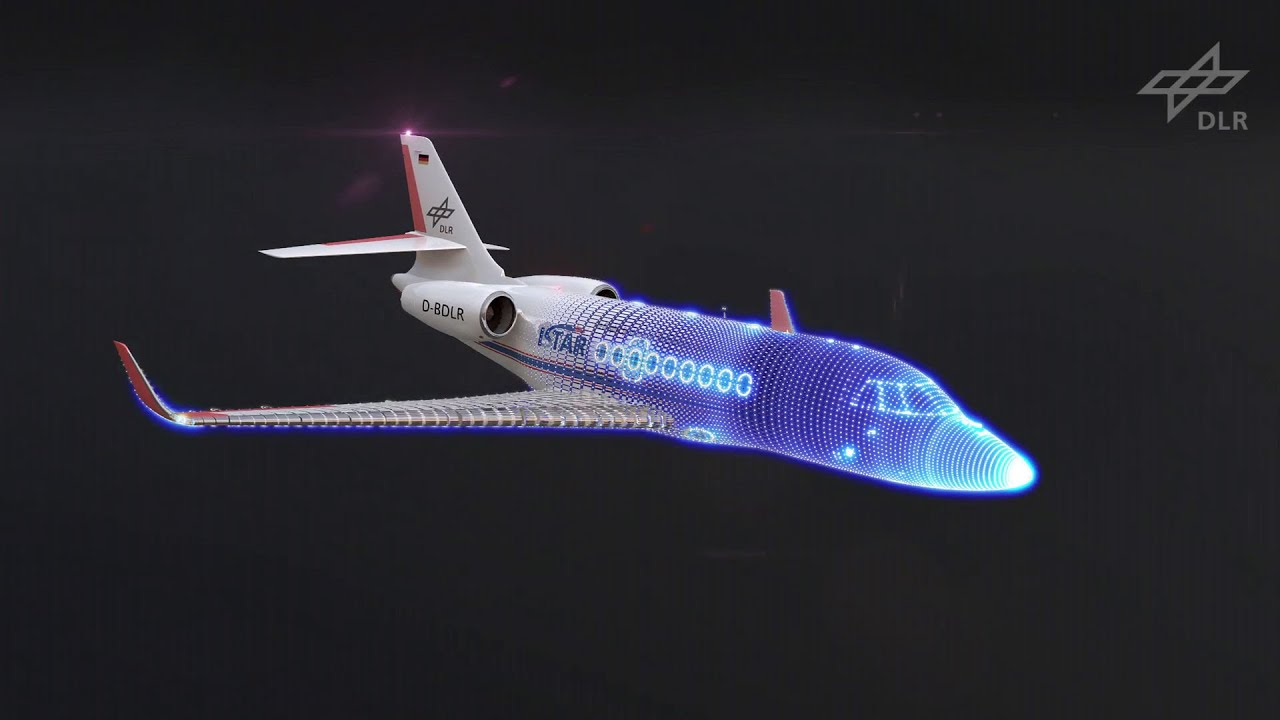
\includegraphics[width=0.7\textwidth]{istar_semitransparent}
    \caption{The ISTARs sensor data systems will be analysed within this work \cite{dlr_dlr-forschungsflugzeug_2020}}
    \ref{fig:istar_semitransparent}
\end{figure}


\section{What}
Q:What is going to be examined within this thesis?
E:The ISTAR aircraft is currently the aircraft generating the most data for the DLR's research aircraft fleet at the Brunswick Research Site. The DLR also owns the largest European fleet of research aircraft, operating 12 aircraft for research purposes ranging from atmospheric research to testing operating limits, pushing the aircraft operating envelope.
-the data acquisitioning system (DAQ) as well as the sensor behaviour is going to be focal point of this work
-also in conjunction with the FAIR principles to allow reusability of the components of this work as well as interoperability with outside algorithms, Accessible due to upload to stash and Findable due to condensing errors into tags and using conventions to catalyze digitalization.

C: examine ISTAR DAQ in detail to detect sensor behaviour anomalies and implement a clear infrastructure to fulfill FAIR principles.


Q: Why is this important?
E:-reduce manual overview of sensors. Currently, much manual postprocessing is needed to get an overview over the large datasets. Large datasets are difficult to work with due to limited computing power. Solving this by working with a Server architecture may be of assistance
-reduce downtime due to sensors. A diagnostic tool for detecting sensor behavior can facilitate the processes and allow a quicker follow up to detect sensor errors since currently system information is distributed and not clearly set
-increase detection rate (sensor faults often not detected). Once a sensor fails during a flight experiment and does not get fixed, the experiment needs to be reflown. This is economically painful since aircraft configurations get customized to experiments needs and the aircraft free slots during a year are low. So a worst case scenario could be that a whole experiment needs to be reflown and a configuration needs to be recustomized and refitted which is a time- and funding intensive task.
-increase reaction time. Often errors are detected weeks after the flight is over. With a software detecting errors directly after sensor data is extracted from the aircraft errors may be detected on the same day. allowing a quicker reaction maybe repeating the experiment during the affixed timeslot.
-build a foundation for a reliability index for sensors. Vital for big data operations within digitalization and the stash project. Should allow for quick implementation of custom data quality algorithms.
-FAIR principles are the new standard within the DLR. Operations however are far from the fulfillment. Documents containing descriptions of sensors and setups are distributed among multiple employees obstructing any efforts to comprehend the already complex aircraft system and its inherent generation of data.
-Safety critical errors may be detected earlier since the proposed routine has potential to go beyond the scope of commercially tested software that is generally employed within aircraft. This software allows a quicker development cycle due to not being bound to the amount of certification aerospace software needs to go through
C:A tool for detection and avoidance of sensor failures is needed to mitigate risks associated with experimental setups since aircraft hours are expensive and the amount of sensors is vast.

\begin{figure}
    \centering
    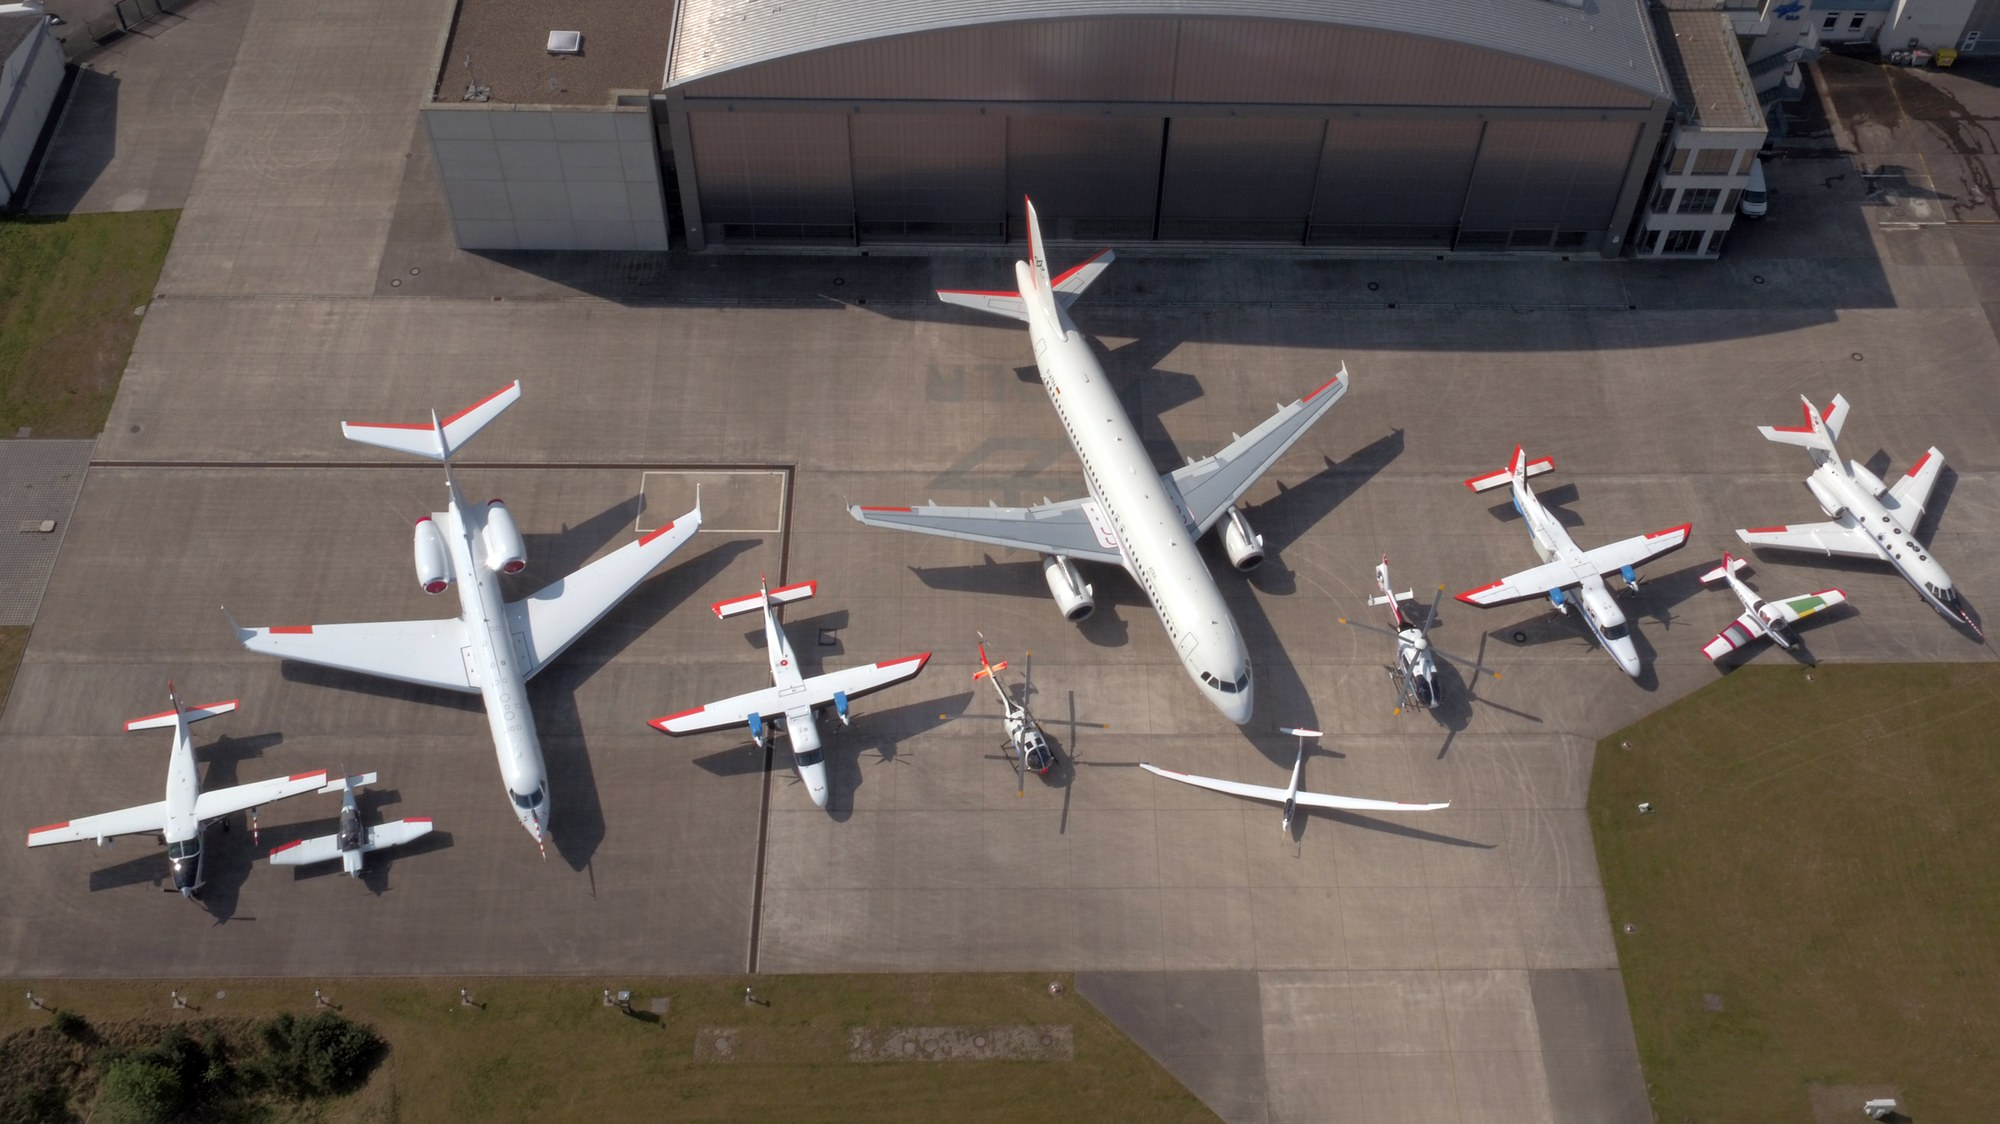
\includegraphics[width=0.7\textwidth]{dlr_fleet.jpeg}
    \caption{The DLRs research fleet without its newest member, a Dornier-228 for Hybrid-Electric Propulsion Research \cite{dlr_dlr-fleet_2018}}
    \ref{fig:dlr_fleet}
\end{figure}

Q:Where does ISTAR data come from?
E:-Generally, the ISTAR has a base DAQ system by IMC co. This base contains inputs from the main aircraft data bus, the experimental nose boom, experimental strain gauges and acc sensors as well as an experimental Inertial Measuring Unit (IMU) combined with a GNSS-System.
-In addition, complementary DAQs may be added to fulfill given experiment requirements.
-ascb bus data originates from various sources, ranging from air data that gets measured by a sensor working on an electric current which then gets transformed by an Analog Digital Converter (ADC) into a digital, discretized signal which then gets fed into the main aircraft bus system (simplified). It then gets transmitted to the IMC DAQ. Trouble is a multifaceted effort within this system.

C: Data originates from all over the aircraft and gets collected in the aircraft experimental DAQ.

\section{Origin}
		○ ISTAR DAQ
		DLR data generation (DAQs) (How Data is checked)

Matthews flowchart(dataflow from sensor voltage through computer-computer-user)
Exemplary for a single sensor.

The ISTARs DAQ records the aircrafts own flight data bus (ASCB, avionics standard communications bus), the experimental Noseboom, an additional GPS unit and various additional strain gauges and acceleration sensors that are distributed across the aircraft. configuration currently is described differently within each sub-group.


		○ Different sensors
		○ Different formats/sources



Q: How to solve this rather extensive problem of SHM?
E:-Fault Detection and Mode Analysis (FMEA) is a common problem in engineering disciplines and everywhere where systems become complex. Literature is rich in this regard, so finding an appropriate solution should be a fesible undertaking
-work on the already working dataspace skystash upon which sensor data is already present
-allow clear software interfaces to facilitate future extensions and modes
-Goal is to allow quick overview over sensor errors.
-further methods presented in chapter 2
C: FMEA is a rich field in which many smart people have already worked on similar problems. A new challenge arises from the implementation into a dynamic digital system also keeping in mind to remain open for new changes and addons.

\section{How}
		 Proposal SHM
		 Detect errors and report them
		○ Check ISTAR Data
Filtering out sensor errors is the goal of this thesis. As described in figure \ref{fig:basic_error} the error can be imagined as a disturbance added upon the original sensor value.



\begin{figure}[ht]
	\centering
	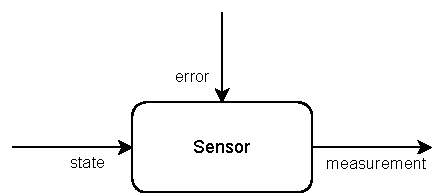
\includegraphics[width=1\textwidth]{basic_error}
	\caption{Sensor Signal}
	\label{fig:basic_error}
\end{figure}

Q: whats the context on this work?
E: this work happens within the DLRs effort to digitize and digitalize the research data and update its research data management strategy.
-Part of DigECat project for ISTAR digital twin
-past work: development of skystash architecture, upload and supply of research data into cloud
-future work: metadata management on a larger scale, metadata frameworks already exists but challenges arise from indexing and providing such large amounts of paper trails in the context of an aircraft. Aircraft are highly complex systems that amass a great amount of paperwork since even its screws require a highly documented certification process.
further big data efforts regarding data analytics allowing for easy scaling of this data base format
-present work: work on prototypes of metadata management to represent sensor data. Calculations then can happen based on datasets with provided metadata without additional inputs.

C: digitalization and digital twin are the companions of this work. A database with data already exists. now it is time to structure metadata allowing for this work to happen dynamically. Building upon this, further metadata may be fed into the system allowing further analytics to be developed.


\paragraph{Conclusion}

This work will examine the sensor data of the ISTAR aircraft, examining various algorithms and methods for FMEA. Then developing a software that allows dynamic implementations of various FMEAs to generate a dynamic backend facilitating development and finally generating reports on data quality for the aircraft systems. FAIR principles are vital for future legibility and exchangeability of data and hence become a central part of this thesis facilitating future use of the results generated within this work.